\documentclass[]{article}
\usepackage{lmodern}
\usepackage{amssymb,amsmath}
\usepackage{ifxetex,ifluatex}
\usepackage{fixltx2e} % provides \textsubscript
\ifnum 0\ifxetex 1\fi\ifluatex 1\fi=0 % if pdftex
  \usepackage[T1]{fontenc}
  \usepackage[utf8]{inputenc}
\else % if luatex or xelatex
  \ifxetex
    \usepackage{mathspec}
  \else
    \usepackage{fontspec}
  \fi
  \defaultfontfeatures{Ligatures=TeX,Scale=MatchLowercase}
\fi
% use upquote if available, for straight quotes in verbatim environments
\IfFileExists{upquote.sty}{\usepackage{upquote}}{}
% use microtype if available
\IfFileExists{microtype.sty}{%
\usepackage{microtype}
\UseMicrotypeSet[protrusion]{basicmath} % disable protrusion for tt fonts
}{}
\usepackage[margin=1in]{geometry}
\usepackage{hyperref}
\hypersetup{unicode=true,
            pdftitle={Assignment 3},
            pdfborder={0 0 0},
            breaklinks=true}
\urlstyle{same}  % don't use monospace font for urls
\usepackage{color}
\usepackage{fancyvrb}
\newcommand{\VerbBar}{|}
\newcommand{\VERB}{\Verb[commandchars=\\\{\}]}
\DefineVerbatimEnvironment{Highlighting}{Verbatim}{commandchars=\\\{\}}
% Add ',fontsize=\small' for more characters per line
\usepackage{framed}
\definecolor{shadecolor}{RGB}{248,248,248}
\newenvironment{Shaded}{\begin{snugshade}}{\end{snugshade}}
\newcommand{\AlertTok}[1]{\textcolor[rgb]{0.94,0.16,0.16}{#1}}
\newcommand{\AnnotationTok}[1]{\textcolor[rgb]{0.56,0.35,0.01}{\textbf{\textit{#1}}}}
\newcommand{\AttributeTok}[1]{\textcolor[rgb]{0.77,0.63,0.00}{#1}}
\newcommand{\BaseNTok}[1]{\textcolor[rgb]{0.00,0.00,0.81}{#1}}
\newcommand{\BuiltInTok}[1]{#1}
\newcommand{\CharTok}[1]{\textcolor[rgb]{0.31,0.60,0.02}{#1}}
\newcommand{\CommentTok}[1]{\textcolor[rgb]{0.56,0.35,0.01}{\textit{#1}}}
\newcommand{\CommentVarTok}[1]{\textcolor[rgb]{0.56,0.35,0.01}{\textbf{\textit{#1}}}}
\newcommand{\ConstantTok}[1]{\textcolor[rgb]{0.00,0.00,0.00}{#1}}
\newcommand{\ControlFlowTok}[1]{\textcolor[rgb]{0.13,0.29,0.53}{\textbf{#1}}}
\newcommand{\DataTypeTok}[1]{\textcolor[rgb]{0.13,0.29,0.53}{#1}}
\newcommand{\DecValTok}[1]{\textcolor[rgb]{0.00,0.00,0.81}{#1}}
\newcommand{\DocumentationTok}[1]{\textcolor[rgb]{0.56,0.35,0.01}{\textbf{\textit{#1}}}}
\newcommand{\ErrorTok}[1]{\textcolor[rgb]{0.64,0.00,0.00}{\textbf{#1}}}
\newcommand{\ExtensionTok}[1]{#1}
\newcommand{\FloatTok}[1]{\textcolor[rgb]{0.00,0.00,0.81}{#1}}
\newcommand{\FunctionTok}[1]{\textcolor[rgb]{0.00,0.00,0.00}{#1}}
\newcommand{\ImportTok}[1]{#1}
\newcommand{\InformationTok}[1]{\textcolor[rgb]{0.56,0.35,0.01}{\textbf{\textit{#1}}}}
\newcommand{\KeywordTok}[1]{\textcolor[rgb]{0.13,0.29,0.53}{\textbf{#1}}}
\newcommand{\NormalTok}[1]{#1}
\newcommand{\OperatorTok}[1]{\textcolor[rgb]{0.81,0.36,0.00}{\textbf{#1}}}
\newcommand{\OtherTok}[1]{\textcolor[rgb]{0.56,0.35,0.01}{#1}}
\newcommand{\PreprocessorTok}[1]{\textcolor[rgb]{0.56,0.35,0.01}{\textit{#1}}}
\newcommand{\RegionMarkerTok}[1]{#1}
\newcommand{\SpecialCharTok}[1]{\textcolor[rgb]{0.00,0.00,0.00}{#1}}
\newcommand{\SpecialStringTok}[1]{\textcolor[rgb]{0.31,0.60,0.02}{#1}}
\newcommand{\StringTok}[1]{\textcolor[rgb]{0.31,0.60,0.02}{#1}}
\newcommand{\VariableTok}[1]{\textcolor[rgb]{0.00,0.00,0.00}{#1}}
\newcommand{\VerbatimStringTok}[1]{\textcolor[rgb]{0.31,0.60,0.02}{#1}}
\newcommand{\WarningTok}[1]{\textcolor[rgb]{0.56,0.35,0.01}{\textbf{\textit{#1}}}}
\usepackage{longtable,booktabs}
\usepackage{graphicx,grffile}
\makeatletter
\def\maxwidth{\ifdim\Gin@nat@width>\linewidth\linewidth\else\Gin@nat@width\fi}
\def\maxheight{\ifdim\Gin@nat@height>\textheight\textheight\else\Gin@nat@height\fi}
\makeatother
% Scale images if necessary, so that they will not overflow the page
% margins by default, and it is still possible to overwrite the defaults
% using explicit options in \includegraphics[width, height, ...]{}
\setkeys{Gin}{width=\maxwidth,height=\maxheight,keepaspectratio}
\IfFileExists{parskip.sty}{%
\usepackage{parskip}
}{% else
\setlength{\parindent}{0pt}
\setlength{\parskip}{6pt plus 2pt minus 1pt}
}
\setlength{\emergencystretch}{3em}  % prevent overfull lines
\providecommand{\tightlist}{%
  \setlength{\itemsep}{0pt}\setlength{\parskip}{0pt}}
\setcounter{secnumdepth}{0}
% Redefines (sub)paragraphs to behave more like sections
\ifx\paragraph\undefined\else
\let\oldparagraph\paragraph
\renewcommand{\paragraph}[1]{\oldparagraph{#1}\mbox{}}
\fi
\ifx\subparagraph\undefined\else
\let\oldsubparagraph\subparagraph
\renewcommand{\subparagraph}[1]{\oldsubparagraph{#1}\mbox{}}
\fi

%%% Use protect on footnotes to avoid problems with footnotes in titles
\let\rmarkdownfootnote\footnote%
\def\footnote{\protect\rmarkdownfootnote}

%%% Change title format to be more compact
\usepackage{titling}

% Create subtitle command for use in maketitle
\newcommand{\subtitle}[1]{
  \posttitle{
    \begin{center}\large#1\end{center}
    }
}

\setlength{\droptitle}{-2em}

  \title{Assignment 3}
    \pretitle{\vspace{\droptitle}\centering\huge}
  \posttitle{\par}
    \author{}
    \preauthor{}\postauthor{}
    \date{}
    \predate{}\postdate{}
  

\begin{document}
\maketitle

\begin{Shaded}
\begin{Highlighting}[]
\KeywordTok{library}\NormalTok{(tidyverse)}
\end{Highlighting}
\end{Shaded}

1.The Titanic dataset records for each person on the ship the passenger
class, age (child or adult), and sex, and whether they survived or not.
In this assignment you will use logistic regression on a training set
(ttrain) to develop a classification rule, and then this rule will be
applied to the test set (ttest).

\begin{Shaded}
\begin{Highlighting}[]
\NormalTok{ttrain <-}\StringTok{ }\KeywordTok{read.csv}\NormalTok{(}\StringTok{"data/ttrain.csv"}\NormalTok{, }\DataTypeTok{header =} \OtherTok{TRUE}\NormalTok{, }\DataTypeTok{row.names =} \DecValTok{1}\NormalTok{)}
\NormalTok{ttest <-}\StringTok{ }\KeywordTok{read.csv}\NormalTok{(}\StringTok{"data/ttest.csv"}\NormalTok{, }\DataTypeTok{header =} \OtherTok{TRUE}\NormalTok{, }\DataTypeTok{row.names =} \DecValTok{1}\NormalTok{)}
\KeywordTok{head}\NormalTok{(ttrain)}
\end{Highlighting}
\end{Shaded}

\begin{verbatim}
##      Class    Sex   Age Survived
## 633    3rd   Male Adult       No
## 1735  Crew   Male Adult      Yes
## 900   Crew   Male Adult       No
## 1941   1st Female Adult      Yes
## 2067   2nd Female Adult      Yes
## 101    1st   Male Adult       No
\end{verbatim}

\begin{enumerate}
\def\labelenumi{(\alph{enumi})}
\tightlist
\item
  Use logistic regression to build a model relating Survived to Class,
  Age and Sex for the training data ttrain.
\end{enumerate}

\begin{Shaded}
\begin{Highlighting}[]
\NormalTok{model <-}\StringTok{ }\KeywordTok{glm}\NormalTok{(Survived }\OperatorTok{~}\StringTok{ }\NormalTok{Class }\OperatorTok{+}\StringTok{ }\NormalTok{Age }\OperatorTok{+}\StringTok{ }\NormalTok{Sex, }\DataTypeTok{data =}\NormalTok{ ttrain, }
             \DataTypeTok{family =} \StringTok{"binomial"}\NormalTok{)}
\KeywordTok{summary}\NormalTok{(model)}
\end{Highlighting}
\end{Shaded}

\begin{verbatim}
## 
## Call:
## glm(formula = Survived ~ Class + Age + Sex, family = "binomial", 
##     data = ttrain)
## 
## Deviance Residuals: 
##     Min       1Q   Median       3Q      Max  
## -2.1232  -0.7173  -0.4496   0.6768   2.1642  
## 
## Coefficients:
##             Estimate Std. Error z value Pr(>|z|)    
## (Intercept)   2.1431     0.1922  11.153  < 2e-16 ***
## Class2nd     -1.0136     0.2219  -4.567 4.95e-06 ***
## Class3rd     -1.8467     0.1952  -9.462  < 2e-16 ***
## ClassCrew    -0.8321     0.1779  -4.678 2.90e-06 ***
## AgeChild      1.0606     0.2889   3.671 0.000242 ***
## SexMale      -2.5373     0.1606 -15.795  < 2e-16 ***
## ---
## Signif. codes:  0 '***' 0.001 '**' 0.01 '*' 0.05 '.' 0.1 ' ' 1
## 
## (Dispersion parameter for binomial family taken to be 1)
## 
##     Null deviance: 2214.5  on 1760  degrees of freedom
## Residual deviance: 1737.6  on 1755  degrees of freedom
## AIC: 1749.6
## 
## Number of Fisher Scoring iterations: 4
\end{verbatim}

\begin{enumerate}
\def\labelenumi{(\alph{enumi})}
\setcounter{enumi}{1}
\tightlist
\item
  From the fitted model, calculate a vector prob of survival
  probabilities and a vector pred of predicted classes, for the training
  data. What proportion of survivors are missclassified? What proportion
  of those who died are missclassified? What proportion of the predicted
  survivors actually survived? What is the overall error rate for the
  training data?
\end{enumerate}

\begin{Shaded}
\begin{Highlighting}[]
\NormalTok{pred_prob <-}\StringTok{ }\KeywordTok{predict}\NormalTok{(model, }\DataTypeTok{type =} \StringTok{"response"}\NormalTok{)}
\NormalTok{ttrain}\OperatorTok{$}\NormalTok{pred_class <-}\StringTok{ }\KeywordTok{ifelse}\NormalTok{(pred_prob }\OperatorTok{<}\StringTok{ }\FloatTok{0.5}\NormalTok{, }\StringTok{"No"}\NormalTok{, }\StringTok{"Yes"}\NormalTok{)}

\CommentTok{# table(ttrain$Survived, pred_class)}

\NormalTok{ttrain }\OperatorTok\StringTok{ }
\StringTok{  }\KeywordTok{group_by}\NormalTok{(pred_class, Survived) }\OperatorTok\StringTok{ }
\StringTok{  }\KeywordTok{count}\NormalTok{() }\OperatorTok\StringTok{ }
\StringTok{  }\KeywordTok{ungroup}\NormalTok{() }\OperatorTok\StringTok{ }
\StringTok{  }\KeywordTok{mutate}\NormalTok{(}\DataTypeTok{perc =}\NormalTok{ scales}\OperatorTok{::}\KeywordTok{percent}\NormalTok{(n}\OperatorTok{/}\KeywordTok{sum}\NormalTok{(n)))}
\end{Highlighting}
\end{Shaded}

\begin{verbatim}
## # A tibble: 4 x 4
##   pred_class Survived     n perc 
##   <chr>      <fct>    <int> <chr>
## 1 No         No        1097 62.3%
## 2 No         Yes        284 16.1%
## 3 Yes        No          96 5.5% 
## 4 Yes        Yes        284 16.1%
\end{verbatim}

\begin{Shaded}
\begin{Highlighting}[]
\CommentTok{# Error = 5.5 + 16.1 = 21.6%}
\end{Highlighting}
\end{Shaded}

\begin{enumerate}
\def\labelenumi{(\alph{enumi})}
\setcounter{enumi}{2}
\tightlist
\item
  From the fitted model, calculate a vector prob of survival
  probabilities and a vector pred of predicted classes, for the test
  data. What proportion of survivors are missclassified? What proportion
  of those who died are missclassified? What proportion of the predicted
  survivors actually survived? What is the overall error rate for the
  test data?
\end{enumerate}

\begin{Shaded}
\begin{Highlighting}[]
\CommentTok{# Probabilities}
\NormalTok{pred_prob_test <-}\StringTok{ }\KeywordTok{predict}\NormalTok{(model, }\DataTypeTok{type =} \StringTok{"response"}\NormalTok{, }\DataTypeTok{newdata =}\NormalTok{ ttest)}
\NormalTok{ttest}\OperatorTok{$}\NormalTok{pred_class <-}\StringTok{ }\KeywordTok{ifelse}\NormalTok{(pred_prob_test }\OperatorTok{<}\StringTok{ }\FloatTok{0.5}\NormalTok{, }\StringTok{"No"}\NormalTok{, }\StringTok{"Yes"}\NormalTok{)}

\KeywordTok{table}\NormalTok{(ttest}\OperatorTok{$}\NormalTok{pred_class, ttest}\OperatorTok{$}\NormalTok{Survived)}
\end{Highlighting}
\end{Shaded}

\begin{verbatim}
##      
##        No Yes
##   No  267  78
##   Yes  30  65
\end{verbatim}

\begin{Shaded}
\begin{Highlighting}[]
\NormalTok{ttest }\OperatorTok\StringTok{ }
\StringTok{  }\KeywordTok{group_by}\NormalTok{(pred_class, Survived) }\OperatorTok\StringTok{ }
\StringTok{  }\KeywordTok{count}\NormalTok{() }\OperatorTok\StringTok{ }
\StringTok{  }\KeywordTok{ungroup}\NormalTok{() }\OperatorTok\StringTok{ }
\StringTok{  }\KeywordTok{mutate}\NormalTok{(}\DataTypeTok{perc =}\NormalTok{ scales}\OperatorTok{::}\KeywordTok{percent}\NormalTok{(n}\OperatorTok{/}\KeywordTok{sum}\NormalTok{(n)))}
\end{Highlighting}
\end{Shaded}

\begin{verbatim}
## # A tibble: 4 x 4
##   pred_class Survived     n perc 
##   <chr>      <fct>    <int> <chr>
## 1 No         No         267 60.7%
## 2 No         Yes         78 17.7%
## 3 Yes        No          30 6.8% 
## 4 Yes        Yes         65 14.8%
\end{verbatim}

\begin{Shaded}
\begin{Highlighting}[]
\CommentTok{# Error = 6.8 + 17.7 = 24.5%}
\end{Highlighting}
\end{Shaded}

\begin{enumerate}
\def\labelenumi{\arabic{enumi}.}
\setcounter{enumi}{1}
\tightlist
\item
  Suppose we wish to predict whether a given stock will issue a dividend
  this year (yes or no) based on X, last year's percentage profit. We
  examine a large number of companies and discover that the mean value
  of X for companies that issued a dividend was 10, while the mean for
  those that didn't was 0. In addition, the variance of X for these two
  sets of companies was 36. Finally, 80\% of companies issued dividends.
  Assuming that X follows a normal distribution, predict the probability
  that a company will issue a dividend this year given that its
  percentage profit was X = 4 last year.
\end{enumerate}

\begin{Shaded}
\begin{Highlighting}[]
\CommentTok{# Probability of issuing dividend }
\NormalTok{p_div <-}\StringTok{ }\FloatTok{0.8}\OperatorTok{*}\KeywordTok{exp}\NormalTok{(}\OperatorTok{-}\StringTok{ }\NormalTok{(}\DecValTok{1}\OperatorTok{/}\DecValTok{72}\NormalTok{) }\OperatorTok{*}\StringTok{ }\NormalTok{(}\DecValTok{4} \OperatorTok{-}\StringTok{ }\DecValTok{10}\NormalTok{)}\OperatorTok{^}\DecValTok{2}\NormalTok{)}
\CommentTok{# Probability of non issuing dividend }
\NormalTok{p_ndiv <-}\StringTok{ }\FloatTok{0.2}\OperatorTok{*}\KeywordTok{exp}\NormalTok{(}\OperatorTok{-}\StringTok{ }\NormalTok{(}\DecValTok{1}\OperatorTok{/}\DecValTok{72}\NormalTok{) }\OperatorTok{*}\StringTok{ }\NormalTok{(}\DecValTok{4} \OperatorTok{-}\StringTok{ }\DecValTok{0}\NormalTok{)}\OperatorTok{^}\DecValTok{2}\NormalTok{)}

\CommentTok{# Result}
\NormalTok{p_div}\OperatorTok{/}\NormalTok{(p_div }\OperatorTok{+}\StringTok{ }\NormalTok{p_ndiv)}
\end{Highlighting}
\end{Shaded}

\begin{verbatim}
## [1] 0.7518525
\end{verbatim}

\begin{enumerate}
\def\labelenumi{\arabic{enumi}.}
\setcounter{enumi}{2}
\tightlist
\item
  In the Auto data, create a new variable that contains the value 1 for
  cars with above the median mpg, and 0 for other cars. Name this
  variable mpg01 Split the data into a test and training sets of size
  containing 50\% and 50\% of observations each.
\end{enumerate}

\begin{Shaded}
\begin{Highlighting}[]
\KeywordTok{library}\NormalTok{(MASS)}
\KeywordTok{library}\NormalTok{(ISLR)}
\KeywordTok{library}\NormalTok{(class)}
\NormalTok{m <-}\StringTok{ }\KeywordTok{median}\NormalTok{(Auto}\OperatorTok{$}\NormalTok{mpg)}
\NormalTok{Auto}\OperatorTok{$}\NormalTok{mpg01 <-}\StringTok{ }\KeywordTok{factor}\NormalTok{(}\KeywordTok{ifelse}\NormalTok{(Auto}\OperatorTok{$}\NormalTok{mpg }\OperatorTok{<=}\StringTok{ }\NormalTok{m, }\DecValTok{0}\NormalTok{, }\DecValTok{1}\NormalTok{))}
\KeywordTok{set.seed}\NormalTok{(}\DecValTok{1}\NormalTok{)}
\NormalTok{s <-}\StringTok{ }\KeywordTok{sample}\NormalTok{(}\KeywordTok{nrow}\NormalTok{(Auto), }\KeywordTok{round}\NormalTok{(.}\DecValTok{5}\OperatorTok{*}\KeywordTok{nrow}\NormalTok{(Auto)))}
\NormalTok{Atrain <-}\StringTok{ }\NormalTok{Auto[s,]}
\NormalTok{Atest <-}\StringTok{ }\NormalTok{Auto[}\OperatorTok{-}\NormalTok{s,]}
\end{Highlighting}
\end{Shaded}

\begin{enumerate}
\def\labelenumi{(\alph{enumi})}
\tightlist
\item
  Plot the variables weight and acceleration using colour to show the
  two levels of mpg01 for the training set.
\end{enumerate}

\begin{Shaded}
\begin{Highlighting}[]
\NormalTok{Atrain }\OperatorTok\StringTok{ }
\StringTok{  }\KeywordTok{ggplot}\NormalTok{(}\KeywordTok{aes}\NormalTok{(weight, acceleration)) }\OperatorTok{+}
\StringTok{  }\KeywordTok{geom_point}\NormalTok{(}\KeywordTok{aes}\NormalTok{(}\DataTypeTok{colour =}\NormalTok{ mpg01)) }\OperatorTok{+}
\StringTok{  }\KeywordTok{theme_bw}\NormalTok{()}
\end{Highlighting}
\end{Shaded}

\begin{center}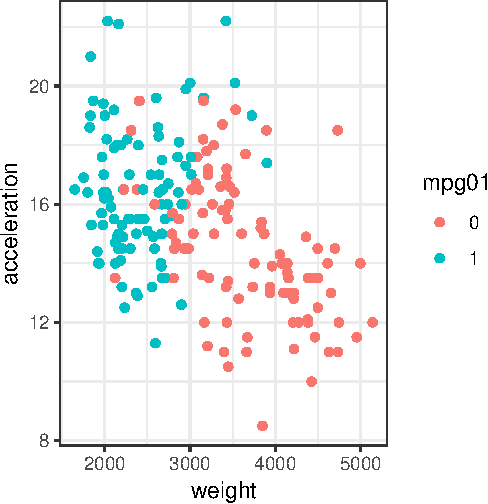
\includegraphics{sol_A3_files/figure-latex/unnamed-chunk-8-1} \end{center}

\begin{enumerate}
\def\labelenumi{(\alph{enumi})}
\setcounter{enumi}{1}
\tightlist
\item
  Perform a linear discriminant analysis to predict mpg01, using
  variables weight and acceleration, on the training set. Use a plot to
  show the discriminant boundaries. What is the test error of the model
  obtained?
\end{enumerate}

\begin{Shaded}
\begin{Highlighting}[]
\NormalTok{lda <-}\StringTok{ }\KeywordTok{lda}\NormalTok{(mpg01 }\OperatorTok{~}\StringTok{ }\NormalTok{weight }\OperatorTok{+}\StringTok{ }\NormalTok{acceleration, }\DataTypeTok{data =}\NormalTok{ Atrain)}
\NormalTok{lda}
\end{Highlighting}
\end{Shaded}

\begin{verbatim}
## Call:
## lda(mpg01 ~ weight + acceleration, data = Atrain)
## 
## Prior probabilities of groups:
##         0         1 
## 0.5255102 0.4744898 
## 
## Group means:
##     weight acceleration
## 0 3636.359     14.49806
## 1 2404.151     16.43226
## 
## Coefficients of linear discriminants:
##                       LD1
## weight       -0.001635093
## acceleration  0.060260084
\end{verbatim}

\begin{Shaded}
\begin{Highlighting}[]
\NormalTok{Atest}\OperatorTok{$}\NormalTok{pred <-}\StringTok{ }\KeywordTok{predict}\NormalTok{(lda, Atest)}\OperatorTok{$}\NormalTok{class}

\NormalTok{Atest }\OperatorTok\StringTok{ }
\StringTok{  }\KeywordTok{group_by}\NormalTok{(pred, mpg01) }\OperatorTok\StringTok{ }
\StringTok{  }\KeywordTok{count}\NormalTok{() }\OperatorTok\StringTok{ }
\StringTok{  }\KeywordTok{ungroup}\NormalTok{() }\OperatorTok\StringTok{ }
\StringTok{  }\KeywordTok{mutate}\NormalTok{(}\DataTypeTok{perc =}\NormalTok{ scales}\OperatorTok{::}\KeywordTok{percent}\NormalTok{(n}\OperatorTok{/}\KeywordTok{sum}\NormalTok{(n)))}
\end{Highlighting}
\end{Shaded}

\begin{verbatim}
## # A tibble: 4 x 4
##   pred  mpg01     n perc 
##   <fct> <fct> <int> <chr>
## 1 0     0        72 36.7%
## 2 0     1         4 2.0% 
## 3 1     0        21 10.7%
## 4 1     1        99 50.5%
\end{verbatim}

\begin{Shaded}
\begin{Highlighting}[]
\CommentTok{# Error = 2 + 10.7 = 12.7%}
\end{Highlighting}
\end{Shaded}

\begin{Shaded}
\begin{Highlighting}[]
\NormalTok{grid <-}\StringTok{ }\KeywordTok{expand.grid}\NormalTok{(}
  \DataTypeTok{weight =} \KeywordTok{seq}\NormalTok{(}\KeywordTok{min}\NormalTok{(Atrain}\OperatorTok{$}\NormalTok{weight), }\KeywordTok{max}\NormalTok{(Atrain}\OperatorTok{$}\NormalTok{weight), }\DataTypeTok{length =} \DecValTok{100}\NormalTok{),}
  \DataTypeTok{acceleration =} \KeywordTok{seq}\NormalTok{(}\KeywordTok{min}\NormalTok{(Atrain}\OperatorTok{$}\NormalTok{acceleration), }\KeywordTok{max}\NormalTok{(Atrain}\OperatorTok{$}\NormalTok{acceleration), }
                     \DataTypeTok{length =} \DecValTok{100}\NormalTok{)}
\NormalTok{)}

\NormalTok{grid}\OperatorTok{$}\NormalTok{pred <-}\StringTok{ }\KeywordTok{predict}\NormalTok{(lda, grid)}\OperatorTok{$}\NormalTok{class}
\KeywordTok{ggplot}\NormalTok{(}\KeywordTok{aes}\NormalTok{(}\DataTypeTok{x =}\NormalTok{ weight, }\DataTypeTok{y =}\NormalTok{ acceleration, }\DataTypeTok{color =}\NormalTok{ pred), }
       \DataTypeTok{data =}\NormalTok{ grid) }\OperatorTok{+}\StringTok{ }
\StringTok{  }\KeywordTok{geom_point}\NormalTok{(}\DataTypeTok{size=}\NormalTok{.}\DecValTok{3}\NormalTok{) }\OperatorTok{+}
\StringTok{  }\KeywordTok{theme_bw}\NormalTok{()}
\end{Highlighting}
\end{Shaded}

\begin{center}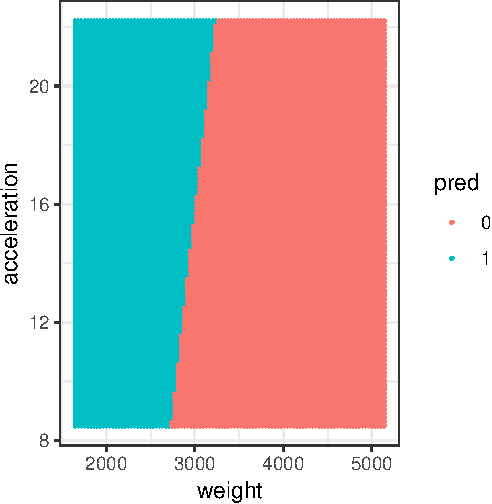
\includegraphics{sol_A3_files/figure-latex/unnamed-chunk-10-1} \end{center}

\begin{enumerate}
\def\labelenumi{(\alph{enumi})}
\setcounter{enumi}{2}
\tightlist
\item
  Repeat (b) using quadratic discriminant analysis. Which is better, LDA
  or QDA?
\end{enumerate}

\begin{Shaded}
\begin{Highlighting}[]
\NormalTok{qda <-}\StringTok{ }\KeywordTok{qda}\NormalTok{(mpg01 }\OperatorTok{~}\StringTok{ }\NormalTok{weight }\OperatorTok{+}\StringTok{ }\NormalTok{acceleration, }\DataTypeTok{data =}\NormalTok{ Atrain)}
\NormalTok{qda}
\end{Highlighting}
\end{Shaded}

\begin{verbatim}
## Call:
## qda(mpg01 ~ weight + acceleration, data = Atrain)
## 
## Prior probabilities of groups:
##         0         1 
## 0.5255102 0.4744898 
## 
## Group means:
##     weight acceleration
## 0 3636.359     14.49806
## 1 2404.151     16.43226
\end{verbatim}

\begin{Shaded}
\begin{Highlighting}[]
\NormalTok{Atest}\OperatorTok{$}\NormalTok{pred <-}\StringTok{ }\KeywordTok{predict}\NormalTok{(qda, Atest)}\OperatorTok{$}\NormalTok{class}

\NormalTok{Atest }\OperatorTok\StringTok{ }
\StringTok{  }\KeywordTok{group_by}\NormalTok{(pred, mpg01) }\OperatorTok\StringTok{ }
\StringTok{  }\KeywordTok{count}\NormalTok{() }\OperatorTok\StringTok{ }
\StringTok{  }\KeywordTok{ungroup}\NormalTok{() }\OperatorTok\StringTok{ }
\StringTok{  }\KeywordTok{mutate}\NormalTok{(}\DataTypeTok{perc =}\NormalTok{ scales}\OperatorTok{::}\KeywordTok{percent}\NormalTok{(n}\OperatorTok{/}\KeywordTok{sum}\NormalTok{(n)))}
\end{Highlighting}
\end{Shaded}

\begin{verbatim}
## # A tibble: 4 x 4
##   pred  mpg01     n perc 
##   <fct> <fct> <int> <chr>
## 1 0     0        71 36.2%
## 2 0     1         2 1.0% 
## 3 1     0        22 11.2%
## 4 1     1       101 51.5%
\end{verbatim}

\begin{Shaded}
\begin{Highlighting}[]
\CommentTok{# Error = 1 + 12.2 = 12.2%}
\end{Highlighting}
\end{Shaded}

\begin{Shaded}
\begin{Highlighting}[]
\NormalTok{grid}\OperatorTok{$}\NormalTok{pred <-}\StringTok{ }\KeywordTok{predict}\NormalTok{(qda, grid)}\OperatorTok{$}\NormalTok{class}
\KeywordTok{ggplot}\NormalTok{(}\KeywordTok{aes}\NormalTok{(}\DataTypeTok{x =}\NormalTok{ weight, }\DataTypeTok{y =}\NormalTok{ acceleration, }\DataTypeTok{color =}\NormalTok{ pred), }
       \DataTypeTok{data =}\NormalTok{ grid) }\OperatorTok{+}\StringTok{ }
\StringTok{  }\KeywordTok{geom_point}\NormalTok{(}\DataTypeTok{size=}\NormalTok{.}\DecValTok{3}\NormalTok{) }\OperatorTok{+}
\StringTok{  }\KeywordTok{theme_bw}\NormalTok{()}
\end{Highlighting}
\end{Shaded}

\begin{center}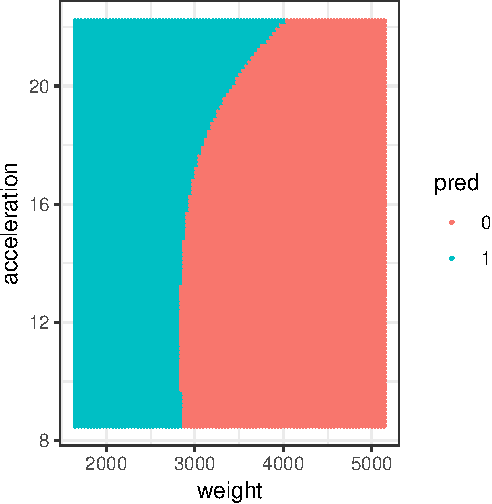
\includegraphics{sol_A3_files/figure-latex/unnamed-chunk-12-1} \end{center}

\begin{enumerate}
\def\labelenumi{(\alph{enumi})}
\setcounter{enumi}{3}
\tightlist
\item
  Perform a linear discriminant analysis to predict mpg01, using
  variables displacement, horsepower, weight and acceleration on the
  training set. What is the test error of the model obtained?
\end{enumerate}

\begin{Shaded}
\begin{Highlighting}[]
\NormalTok{lda <-}\StringTok{ }\KeywordTok{lda}\NormalTok{(mpg01 }\OperatorTok{~}\StringTok{ }\NormalTok{displacement }\OperatorTok{+}\StringTok{ }\NormalTok{horsepower }\OperatorTok{+}\StringTok{ }
\StringTok{           }\NormalTok{weight }\OperatorTok{+}\StringTok{ }\NormalTok{acceleration, }\DataTypeTok{data =}\NormalTok{ Atrain)}
\NormalTok{lda}
\end{Highlighting}
\end{Shaded}

\begin{verbatim}
## Call:
## lda(mpg01 ~ displacement + horsepower + weight + acceleration, 
##     data = Atrain)
## 
## Prior probabilities of groups:
##         0         1 
## 0.5255102 0.4744898 
## 
## Group means:
##   displacement horsepower   weight acceleration
## 0     272.6214  131.69903 3636.359     14.49806
## 1     123.9140   80.11828 2404.151     16.43226
## 
## Coefficients of linear discriminants:
##                        LD1
## displacement -0.0055437546
## horsepower   -0.0039716637
## weight       -0.0009141395
## acceleration  0.0086776698
\end{verbatim}

\begin{Shaded}
\begin{Highlighting}[]
\NormalTok{Atest}\OperatorTok{$}\NormalTok{pred <-}\StringTok{ }\KeywordTok{predict}\NormalTok{(lda, Atest)}\OperatorTok{$}\NormalTok{class}

\NormalTok{Atest }\OperatorTok\StringTok{ }
\StringTok{  }\KeywordTok{group_by}\NormalTok{(pred, mpg01) }\OperatorTok\StringTok{ }
\StringTok{  }\KeywordTok{count}\NormalTok{() }\OperatorTok\StringTok{ }
\StringTok{  }\KeywordTok{ungroup}\NormalTok{() }\OperatorTok\StringTok{ }
\StringTok{  }\KeywordTok{mutate}\NormalTok{(}\DataTypeTok{perc =}\NormalTok{ scales}\OperatorTok{::}\KeywordTok{percent}\NormalTok{(n}\OperatorTok{/}\KeywordTok{sum}\NormalTok{(n)))}
\end{Highlighting}
\end{Shaded}

\begin{verbatim}
## # A tibble: 3 x 4
##   pred  mpg01     n perc 
##   <fct> <fct> <int> <chr>
## 1 0     0        73 37.2%
## 2 1     0        20 10.2%
## 3 1     1       103 52.6%
\end{verbatim}

\begin{Shaded}
\begin{Highlighting}[]
\CommentTok{# Error = 10.2%}
\end{Highlighting}
\end{Shaded}

\begin{enumerate}
\def\labelenumi{(\alph{enumi})}
\setcounter{enumi}{4}
\tightlist
\item
  Repeat (d) using quadratic discriminant analysis. Which is better, LDA
  or QDA?
\end{enumerate}

\begin{Shaded}
\begin{Highlighting}[]
\NormalTok{qda <-}\StringTok{ }\KeywordTok{qda}\NormalTok{(mpg01 }\OperatorTok{~}\StringTok{ }\NormalTok{displacement }\OperatorTok{+}\StringTok{ }\NormalTok{horsepower }\OperatorTok{+}\StringTok{ }
\StringTok{           }\NormalTok{weight }\OperatorTok{+}\StringTok{ }\NormalTok{acceleration, }\DataTypeTok{data =}\NormalTok{ Atrain)}
\NormalTok{qda}
\end{Highlighting}
\end{Shaded}

\begin{verbatim}
## Call:
## qda(mpg01 ~ displacement + horsepower + weight + acceleration, 
##     data = Atrain)
## 
## Prior probabilities of groups:
##         0         1 
## 0.5255102 0.4744898 
## 
## Group means:
##   displacement horsepower   weight acceleration
## 0     272.6214  131.69903 3636.359     14.49806
## 1     123.9140   80.11828 2404.151     16.43226
\end{verbatim}

\begin{Shaded}
\begin{Highlighting}[]
\NormalTok{Atest}\OperatorTok{$}\NormalTok{pred <-}\StringTok{ }\KeywordTok{predict}\NormalTok{(qda, Atest)}\OperatorTok{$}\NormalTok{class}

\NormalTok{Atest }\OperatorTok\StringTok{ }
\StringTok{  }\KeywordTok{group_by}\NormalTok{(pred, mpg01) }\OperatorTok\StringTok{ }
\StringTok{  }\KeywordTok{count}\NormalTok{() }\OperatorTok\StringTok{ }
\StringTok{  }\KeywordTok{ungroup}\NormalTok{() }\OperatorTok\StringTok{ }
\StringTok{  }\KeywordTok{mutate}\NormalTok{(}\DataTypeTok{perc =}\NormalTok{ scales}\OperatorTok{::}\KeywordTok{percent}\NormalTok{(n}\OperatorTok{/}\KeywordTok{sum}\NormalTok{(n)))}
\end{Highlighting}
\end{Shaded}

\begin{verbatim}
## # A tibble: 4 x 4
##   pred  mpg01     n perc 
##   <fct> <fct> <int> <chr>
## 1 0     0        75 38.3%
## 2 0     1         6 3.1% 
## 3 1     0        18 9.2% 
## 4 1     1        97 49.5%
\end{verbatim}

\begin{Shaded}
\begin{Highlighting}[]
\CommentTok{# Error = 3.1 + 9.2 = 12.3 %}
\end{Highlighting}
\end{Shaded}

\begin{enumerate}
\def\labelenumi{(\alph{enumi})}
\setcounter{enumi}{5}
\tightlist
\item
  Perform KNN with response of mpg01, and the four predictors
  displacement, horsepower, weight and acceleration. Remember to scale
  the predictors. Use k = 5 and k = 30. Which value of k gives the best
  result on the test set?
\end{enumerate}

\begin{Shaded}
\begin{Highlighting}[]
\NormalTok{scaled_train <-}\StringTok{   }\NormalTok{Atrain }\OperatorTok\StringTok{  }
\StringTok{    }\NormalTok{dplyr}\OperatorTok{::}\KeywordTok{select}\NormalTok{(displacement, horsepower, weight, acceleration) }\OperatorTok\StringTok{ }
\StringTok{    }\KeywordTok{mutate_all}\NormalTok{(scale)}

\NormalTok{scaled_test <-}\StringTok{   }\NormalTok{Atest }\OperatorTok\StringTok{  }
\StringTok{    }\NormalTok{dplyr}\OperatorTok{::}\KeywordTok{select}\NormalTok{(displacement, horsepower, weight, acceleration) }\OperatorTok\StringTok{ }
\StringTok{    }\KeywordTok{mutate_all}\NormalTok{(scale)}

\NormalTok{knn_}\DecValTok{5}\NormalTok{ <-}\StringTok{ }\KeywordTok{knn}\NormalTok{(}
\NormalTok{  scaled_train,}
\NormalTok{  scaled_test, }
  \DataTypeTok{cl =}\NormalTok{ Atrain}\OperatorTok{$}\NormalTok{mpg01,}
  \DataTypeTok{k =} \DecValTok{5}\NormalTok{)}

\NormalTok{knn_}\DecValTok{30}\NormalTok{ <-}\StringTok{ }\KeywordTok{knn}\NormalTok{(}
\NormalTok{  scaled_train,}
\NormalTok{  scaled_test, }
  \DataTypeTok{cl =}\NormalTok{ Atrain}\OperatorTok{$}\NormalTok{mpg01,}
  \DataTypeTok{k =} \DecValTok{30}\NormalTok{)}

\KeywordTok{table}\NormalTok{(Atest}\OperatorTok{$}\NormalTok{mpg01, knn_}\DecValTok{5}\NormalTok{)}
\end{Highlighting}
\end{Shaded}

\begin{verbatim}
##    knn_5
##      0  1
##   0 81 12
##   1  7 96
\end{verbatim}

\begin{Shaded}
\begin{Highlighting}[]
\KeywordTok{table}\NormalTok{(Atest}\OperatorTok{$}\NormalTok{mpg01, knn_}\DecValTok{30}\NormalTok{)}
\end{Highlighting}
\end{Shaded}

\begin{verbatim}
##    knn_30
##      0  1
##   0 81 12
##   1  8 95
\end{verbatim}

\begin{enumerate}
\def\labelenumi{\arabic{enumi}.}
\setcounter{enumi}{3}
\tightlist
\item
  A classifier gives the following result. In the table below, Group
  gives the true class, and Prob gives the estimated probability of
  Group A (positive) using the classifier.
\end{enumerate}

\begin{Shaded}
\begin{Highlighting}[]
\NormalTok{groups <-}\StringTok{ }\KeywordTok{data.frame}\NormalTok{(}
  \DataTypeTok{group =} \KeywordTok{c}\NormalTok{(}\KeywordTok{rep}\NormalTok{(}\StringTok{"A"}\NormalTok{, }\DataTypeTok{each =} \DecValTok{6}\NormalTok{), }\KeywordTok{rep}\NormalTok{(}\StringTok{"B"}\NormalTok{, }\DataTypeTok{each =} \DecValTok{4}\NormalTok{)),}
  \DataTypeTok{p =} \KeywordTok{c}\NormalTok{(}\FloatTok{0.206}\NormalTok{, }\FloatTok{0.177}\NormalTok{, }\FloatTok{0.687}\NormalTok{, }\FloatTok{0.384}\NormalTok{, }\FloatTok{0.770}\NormalTok{, }\FloatTok{0.498}\NormalTok{, }\FloatTok{0.718}\NormalTok{, }
        \FloatTok{0.992}\NormalTok{, }\FloatTok{0.380}\NormalTok{, }\FloatTok{0.777}\NormalTok{)}
\NormalTok{)}
\NormalTok{groups }\OperatorTok\StringTok{ }\NormalTok{knitr}\OperatorTok{::}\KeywordTok{kable}\NormalTok{()}
\end{Highlighting}
\end{Shaded}

\begin{longtable}[]{@{}lr@{}}
\toprule
group & p\tabularnewline
\midrule
\endhead
A & 0.206\tabularnewline
A & 0.177\tabularnewline
A & 0.687\tabularnewline
A & 0.384\tabularnewline
A & 0.770\tabularnewline
A & 0.498\tabularnewline
B & 0.718\tabularnewline
B & 0.992\tabularnewline
B & 0.380\tabularnewline
B & 0.777\tabularnewline
\bottomrule
\end{longtable}

\begin{enumerate}
\def\labelenumi{(\alph{enumi})}
\tightlist
\item
  What are the predicted classes? Use a threshold of 0.5.
\end{enumerate}

\begin{Shaded}
\begin{Highlighting}[]
\NormalTok{groups <-}\StringTok{ }\NormalTok{groups }\OperatorTok\StringTok{ }
\StringTok{  }\KeywordTok{mutate}\NormalTok{(}\DataTypeTok{pred =} \KeywordTok{ifelse}\NormalTok{(p }\OperatorTok{>}\StringTok{ }\FloatTok{0.5}\NormalTok{, }\StringTok{"A"}\NormalTok{, }\StringTok{"B"}\NormalTok{))}
\end{Highlighting}
\end{Shaded}

\begin{enumerate}
\def\labelenumi{(\alph{enumi})}
\setcounter{enumi}{1}
\tightlist
\item
  What is the error rate? What is the false positive rate? The true
  positive rate?
\end{enumerate}

\begin{Shaded}
\begin{Highlighting}[]
\NormalTok{groups }\OperatorTok\StringTok{ }
\StringTok{  }\KeywordTok{group_by}\NormalTok{(pred, group) }\OperatorTok\StringTok{ }
\StringTok{  }\KeywordTok{count}\NormalTok{() }\OperatorTok\StringTok{ }
\StringTok{  }\KeywordTok{ungroup}\NormalTok{() }\OperatorTok\StringTok{ }
\StringTok{  }\KeywordTok{mutate}\NormalTok{(}\DataTypeTok{perc =}\NormalTok{ scales}\OperatorTok{::}\KeywordTok{percent}\NormalTok{(n}\OperatorTok{/}\KeywordTok{sum}\NormalTok{(n)))}
\end{Highlighting}
\end{Shaded}

\begin{verbatim}
## # A tibble: 4 x 4
##   pred  group     n perc 
##   <chr> <fct> <int> <chr>
## 1 A     A         2 20.0%
## 2 A     B         3 30.0%
## 3 B     A         4 40.0%
## 4 B     B         1 10.0%
\end{verbatim}

\begin{Shaded}
\begin{Highlighting}[]
\CommentTok{# Error = 30 + 40 = 70%}
\end{Highlighting}
\end{Shaded}

\begin{enumerate}
\def\labelenumi{(\alph{enumi})}
\setcounter{enumi}{2}
\tightlist
\item
  Now let the threshold take values 0, .2, .4,.6,.8,1. For each
  threshold calculate the false positive rate, and the true positive
  rate. (If doing this in R use more thresholds.)
\end{enumerate}

\begin{Shaded}
\begin{Highlighting}[]
\NormalTok{trs <-}\StringTok{ }\KeywordTok{seq}\NormalTok{(}\DecValTok{0}\NormalTok{, }\DecValTok{1}\NormalTok{, }\DataTypeTok{by =} \FloatTok{0.05}\NormalTok{)}
\NormalTok{fc <-}\StringTok{ }\ControlFlowTok{function}\NormalTok{(trs)\{}
\NormalTok{  res <-}\StringTok{ }\NormalTok{groups }\OperatorTok\StringTok{ }
\StringTok{    }\KeywordTok{mutate}\NormalTok{(}\DataTypeTok{pred =} \KeywordTok{ifelse}\NormalTok{(p }\OperatorTok{>}\StringTok{ }\NormalTok{trs, }\StringTok{"A"}\NormalTok{, }\StringTok{"B"}\NormalTok{)) }
\NormalTok{  tab <-}\StringTok{ }\KeywordTok{c}\NormalTok{(}\KeywordTok{prop.table}\NormalTok{(}\KeywordTok{table}\NormalTok{(res}\OperatorTok{$}\NormalTok{pred, res}\OperatorTok{$}\NormalTok{group)))}
  
  \ControlFlowTok{while}\NormalTok{(}\KeywordTok{length}\NormalTok{(tab) }\OperatorTok{<}\StringTok{ }\DecValTok{4}\NormalTok{)\{}
\NormalTok{    tab <-}\StringTok{ }\KeywordTok{c}\NormalTok{(tab, }\DecValTok{0}\NormalTok{)  }
\NormalTok{  \}}
\NormalTok{  tab <-}\StringTok{ }\KeywordTok{matrix}\NormalTok{(tab, }\DataTypeTok{ncol =} \DecValTok{2}\NormalTok{, }\DataTypeTok{nrow =} \DecValTok{2}\NormalTok{, }\DataTypeTok{byrow =} \OtherTok{TRUE}\NormalTok{)}
\NormalTok{  tp <-}\StringTok{ }\NormalTok{tab[}\DecValTok{1}\NormalTok{,}\DecValTok{1}\NormalTok{]}
\NormalTok{  fp <-}\StringTok{  }\NormalTok{tab[}\DecValTok{2}\NormalTok{, }\DecValTok{1}\NormalTok{]}
  \KeywordTok{return}\NormalTok{(}\KeywordTok{list}\NormalTok{(}\DataTypeTok{tp =}\NormalTok{ tp, }\DataTypeTok{fp =}\NormalTok{ fp))}
  
\NormalTok{\}}

\NormalTok{res <-}\StringTok{  }\NormalTok{trs }\OperatorTok\StringTok{ }\NormalTok{purrr}\OperatorTok{::}\KeywordTok{map}\NormalTok{(fc) }
\NormalTok{df <-}\StringTok{ }\KeywordTok{data.frame}\NormalTok{(}\DataTypeTok{fp =}\NormalTok{ res }\OperatorTok\StringTok{ }\KeywordTok{map_dbl}\NormalTok{(}\StringTok{"fp"}\NormalTok{),}
                 \DataTypeTok{tp =}\NormalTok{ res }\OperatorTok\StringTok{ }\KeywordTok{map_dbl}\NormalTok{(}\StringTok{"tp"}\NormalTok{))}
\end{Highlighting}
\end{Shaded}

\begin{enumerate}
\def\labelenumi{(\alph{enumi})}
\setcounter{enumi}{3}
\tightlist
\item
  Plot the true positive rate versus the false positive rate. This is
  the ROC curve.
\end{enumerate}

\begin{Shaded}
\begin{Highlighting}[]
\NormalTok{df }\OperatorTok\StringTok{ }
\StringTok{  }\KeywordTok{ggplot}\NormalTok{(}\KeywordTok{aes}\NormalTok{(tp, fp)) }\OperatorTok{+}
\StringTok{  }\KeywordTok{geom_line}\NormalTok{() }\OperatorTok{+}
\StringTok{  }\KeywordTok{labs}\NormalTok{(}\DataTypeTok{y =} \StringTok{"False Positive"}\NormalTok{, }\DataTypeTok{x =} \StringTok{"True Positive"}\NormalTok{)}
\end{Highlighting}
\end{Shaded}

\begin{center}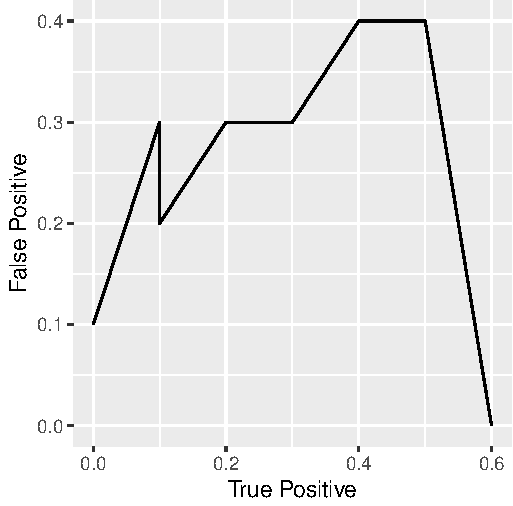
\includegraphics{sol_A3_files/figure-latex/unnamed-chunk-20-1} \end{center}

\begin{enumerate}
\def\labelenumi{(\alph{enumi})}
\setcounter{enumi}{4}
\tightlist
\item
  (Optional, if doing in R) Another classifier just assigns class
  probabilities randomly, ie the estimated probabilities are: Plot the
  ROC curve for this classifier.
\end{enumerate}

\begin{enumerate}
\def\labelenumi{\arabic{enumi}.}
\setcounter{enumi}{4}
\tightlist
\item
  Dataset on diabetes in Pima Indian Women in library(MASS). For a
  description of the data see ?Pima.tr.
\end{enumerate}

Use any supervised classification technique to predict diabetes from the
7 available features. Train your algorithms on Pima.tr and present the
overall error rate for the test data Pima.te.

\begin{enumerate}
\def\labelenumi{\arabic{enumi}.}
\setcounter{enumi}{5}
\tightlist
\item
  Generate some fake data using the following code:
\end{enumerate}

\begin{Shaded}
\begin{Highlighting}[]
\KeywordTok{set.seed}\NormalTok{(}\DecValTok{1}\NormalTok{)}
\NormalTok{x <-}\StringTok{ }\KeywordTok{rnorm}\NormalTok{(}\DecValTok{100}\NormalTok{)}
\NormalTok{y <-}\StringTok{ }\DecValTok{1} \OperatorTok{+}\StringTok{ }\FloatTok{.2}\OperatorTok{*}\NormalTok{x}\OperatorTok{+}\DecValTok{3}\OperatorTok{*}\NormalTok{x}\OperatorTok{^}\DecValTok{2}\FloatTok{+.6}\OperatorTok{*}\NormalTok{x}\OperatorTok{^}\DecValTok{3} \OperatorTok{+}\StringTok{ }\KeywordTok{rnorm}\NormalTok{(}\DecValTok{100}\NormalTok{)}
\NormalTok{d <-}\StringTok{ }\KeywordTok{data.frame}\NormalTok{(}\DataTypeTok{x =}\NormalTok{ x, }\DataTypeTok{y =}\NormalTok{ y)}

\NormalTok{d <-}\StringTok{ }\NormalTok{purrr}\OperatorTok{::}\KeywordTok{map}\NormalTok{(}\DecValTok{2}\OperatorTok{:}\DecValTok{10}\NormalTok{, }
                \OperatorTok{~}\NormalTok{\{ d}\OperatorTok{$}\NormalTok{x}\OperatorTok{^}\NormalTok{.x \}    }
\NormalTok{) }\OperatorTok\StringTok{ }\KeywordTok{bind_cols}\NormalTok{() }\OperatorTok\StringTok{ }
\StringTok{  }\KeywordTok{bind_cols}\NormalTok{(d)}

\CommentTok{# or}

\CommentTok{# for(i in 2:10)\{}
\CommentTok{#   d[ , paste("var", i)] <- d$x^i}
\CommentTok{# }
\CommentTok{# \}}
\end{Highlighting}
\end{Shaded}

Use best subset selection to choose the best model containing predictors
\(X, X^2, \dots, X^{10}\). Which terms are included in the best 3
variable model?

\begin{Shaded}
\begin{Highlighting}[]
\KeywordTok{library}\NormalTok{(leaps)}
\NormalTok{allfits <-}\StringTok{ }\KeywordTok{regsubsets}\NormalTok{(y }\OperatorTok{~}\StringTok{ }\NormalTok{., }\DataTypeTok{data =}\NormalTok{ d)}
\KeywordTok{summary}\NormalTok{(allfits)}\OperatorTok{$}\NormalTok{which}
\end{Highlighting}
\end{Shaded}

\begin{verbatim}
##   (Intercept)   V1    V2    V3    V4    V5    V6    V7    V8    V9     x
## 1        TRUE TRUE FALSE FALSE FALSE FALSE FALSE FALSE FALSE FALSE FALSE
## 2        TRUE TRUE  TRUE FALSE FALSE FALSE FALSE FALSE FALSE FALSE FALSE
## 3        TRUE TRUE FALSE FALSE  TRUE FALSE FALSE FALSE FALSE FALSE  TRUE
## 4        TRUE TRUE  TRUE FALSE  TRUE FALSE FALSE FALSE FALSE FALSE  TRUE
## 5        TRUE TRUE FALSE FALSE  TRUE FALSE FALSE  TRUE  TRUE FALSE  TRUE
## 6        TRUE TRUE  TRUE FALSE FALSE FALSE  TRUE  TRUE  TRUE FALSE  TRUE
## 7        TRUE TRUE FALSE  TRUE  TRUE  TRUE FALSE  TRUE FALSE  TRUE  TRUE
## 8        TRUE TRUE  TRUE  TRUE FALSE  TRUE FALSE  TRUE  TRUE  TRUE  TRUE
\end{verbatim}

\begin{enumerate}
\def\labelenumi{(\alph{enumi})}
\setcounter{enumi}{1}
\tightlist
\item
  Make a plot of \(C^p\) versus number of predictors for the models in
  all fits. Which model has the lowest \(C^p\)? What are its predictors?
\end{enumerate}

\begin{Shaded}
\begin{Highlighting}[]
\KeywordTok{par}\NormalTok{(}\DataTypeTok{mar =} \KeywordTok{c}\NormalTok{(}\DecValTok{3}\NormalTok{,}\DecValTok{3}\NormalTok{,}\DecValTok{0}\NormalTok{,}\DecValTok{0}\NormalTok{))}
\KeywordTok{plot}\NormalTok{(allfits, }\DataTypeTok{scale =} \StringTok{"r2"}\NormalTok{, }\DataTypeTok{col =} \StringTok{"blue"}\NormalTok{, }\DataTypeTok{main =} \StringTok{"Best"}\NormalTok{)}
\end{Highlighting}
\end{Shaded}

\begin{center}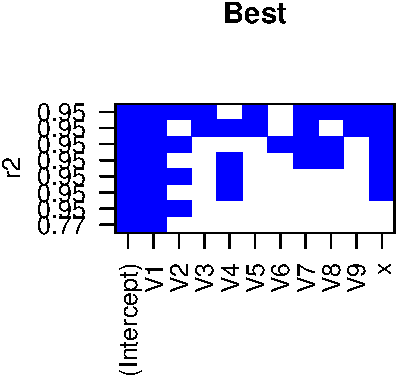
\includegraphics{sol_A3_files/figure-latex/unnamed-chunk-23-1} \end{center}

\begin{Shaded}
\begin{Highlighting}[]
\NormalTok{npred <-}\DecValTok{1}\OperatorTok{:}\DecValTok{8}

\KeywordTok{data.frame}\NormalTok{(}\DataTypeTok{npred =} \DecValTok{1}\OperatorTok{:}\DecValTok{8}\NormalTok{, }
           \DataTypeTok{cp =} \KeywordTok{summary}\NormalTok{(allfits)}\OperatorTok{$}\NormalTok{cp) }\OperatorTok\StringTok{ }
\StringTok{  }\KeywordTok{ggplot}\NormalTok{(}\KeywordTok{aes}\NormalTok{(npred, cp)) }\OperatorTok{+}
\StringTok{  }\KeywordTok{geom_line}\NormalTok{(}\DataTypeTok{colour =} \StringTok{"blue"}\NormalTok{) }\OperatorTok{+}
\StringTok{  }\KeywordTok{geom_point}\NormalTok{() }\OperatorTok{+}\StringTok{ }
\StringTok{  }\KeywordTok{theme_bw}\NormalTok{()}
\end{Highlighting}
\end{Shaded}

\begin{center}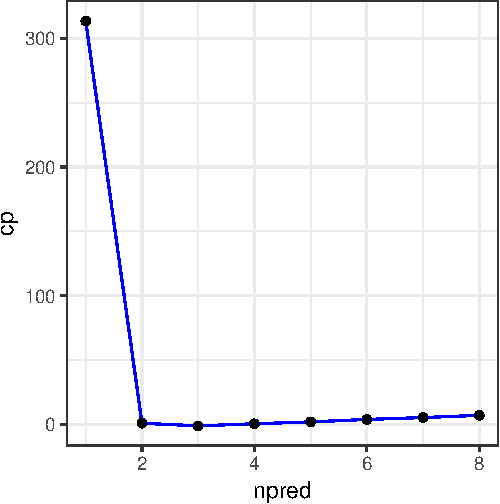
\includegraphics{sol_A3_files/figure-latex/unnamed-chunk-23-2} \end{center}

\begin{enumerate}
\def\labelenumi{(\alph{enumi})}
\setcounter{enumi}{2}
\tightlist
\item
  Reconstruct all fits with option method = ''forward''. Which model has
  the lowest \(C^p\)? What are its predictors?
\end{enumerate}

\begin{Shaded}
\begin{Highlighting}[]
\NormalTok{forw <-}\StringTok{ }\KeywordTok{regsubsets}\NormalTok{(y }\OperatorTok{~}\StringTok{ }\NormalTok{., }\DataTypeTok{data =}\NormalTok{ d, }\DataTypeTok{method=}\StringTok{"forward"}\NormalTok{)}
\KeywordTok{summary}\NormalTok{(forw)}\OperatorTok{$}\NormalTok{which}
\end{Highlighting}
\end{Shaded}

\begin{verbatim}
##   (Intercept)   V1    V2    V3    V4    V5    V6    V7    V8    V9     x
## 1        TRUE TRUE FALSE FALSE FALSE FALSE FALSE FALSE FALSE FALSE FALSE
## 2        TRUE TRUE  TRUE FALSE FALSE FALSE FALSE FALSE FALSE FALSE FALSE
## 3        TRUE TRUE  TRUE FALSE FALSE FALSE FALSE  TRUE FALSE FALSE FALSE
## 4        TRUE TRUE  TRUE FALSE FALSE FALSE FALSE  TRUE FALSE FALSE  TRUE
## 5        TRUE TRUE  TRUE FALSE  TRUE FALSE FALSE  TRUE FALSE FALSE  TRUE
## 6        TRUE TRUE  TRUE FALSE  TRUE FALSE FALSE  TRUE  TRUE FALSE  TRUE
## 7        TRUE TRUE  TRUE FALSE  TRUE FALSE  TRUE  TRUE  TRUE FALSE  TRUE
## 8        TRUE TRUE  TRUE FALSE  TRUE  TRUE  TRUE  TRUE  TRUE FALSE  TRUE
\end{verbatim}

\begin{Shaded}
\begin{Highlighting}[]
\KeywordTok{plot}\NormalTok{(forw, }\DataTypeTok{scale =} \StringTok{"r2"}\NormalTok{, }\DataTypeTok{col =} \StringTok{"blue"}\NormalTok{, }\DataTypeTok{main =} \StringTok{"Best"}\NormalTok{)}
\end{Highlighting}
\end{Shaded}

\begin{center}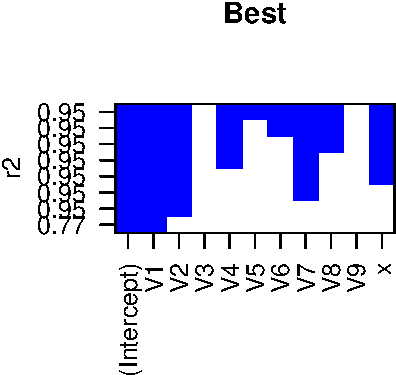
\includegraphics{sol_A3_files/figure-latex/unnamed-chunk-24-1} \end{center}

\begin{Shaded}
\begin{Highlighting}[]
\KeywordTok{data.frame}\NormalTok{(}\DataTypeTok{npred =} \DecValTok{1}\OperatorTok{:}\DecValTok{8}\NormalTok{, }
           \DataTypeTok{cp =} \KeywordTok{summary}\NormalTok{(forw)}\OperatorTok{$}\NormalTok{cp) }\OperatorTok\StringTok{ }
\StringTok{  }\KeywordTok{ggplot}\NormalTok{(}\KeywordTok{aes}\NormalTok{(npred, cp)) }\OperatorTok{+}
\StringTok{  }\KeywordTok{geom_line}\NormalTok{(}\DataTypeTok{colour =} \StringTok{"blue"}\NormalTok{) }\OperatorTok{+}
\StringTok{  }\KeywordTok{geom_point}\NormalTok{() }\OperatorTok{+}\StringTok{ }
\StringTok{  }\KeywordTok{theme_bw}\NormalTok{()}
\end{Highlighting}
\end{Shaded}

\begin{center}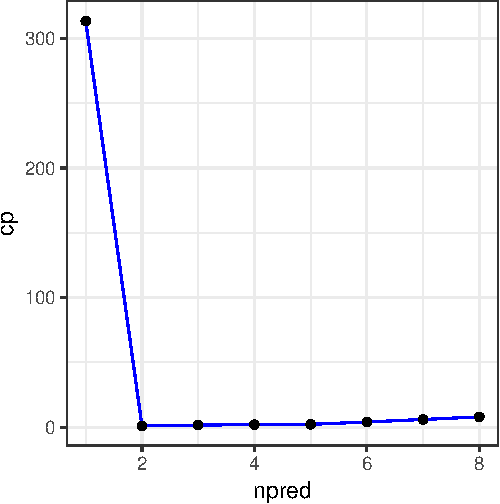
\includegraphics{sol_A3_files/figure-latex/unnamed-chunk-24-2} \end{center}

\begin{enumerate}
\def\labelenumi{(\alph{enumi})}
\setcounter{enumi}{3}
\tightlist
\item
  Reconstruct allfits with option method = ''backward''. Which model has
  the lowest \(C^p\)? What are its predictors?
\end{enumerate}

\begin{Shaded}
\begin{Highlighting}[]
\NormalTok{back <-}\StringTok{ }\KeywordTok{regsubsets}\NormalTok{(y }\OperatorTok{~}\StringTok{ }\NormalTok{., }\DataTypeTok{data =}\NormalTok{ d, }\DataTypeTok{method=}\StringTok{"backward"}\NormalTok{)}
\KeywordTok{summary}\NormalTok{(back)}\OperatorTok{$}\NormalTok{which}
\end{Highlighting}
\end{Shaded}

\begin{verbatim}
##   (Intercept)   V1    V2    V3    V4    V5    V6    V7    V8    V9     x
## 1        TRUE TRUE FALSE FALSE FALSE FALSE FALSE FALSE FALSE FALSE FALSE
## 2        TRUE TRUE FALSE FALSE  TRUE FALSE FALSE FALSE FALSE FALSE FALSE
## 3        TRUE TRUE FALSE FALSE  TRUE FALSE FALSE FALSE FALSE FALSE  TRUE
## 4        TRUE TRUE FALSE FALSE  TRUE FALSE FALSE  TRUE FALSE FALSE  TRUE
## 5        TRUE TRUE FALSE FALSE  TRUE FALSE FALSE  TRUE FALSE  TRUE  TRUE
## 6        TRUE TRUE FALSE FALSE  TRUE  TRUE FALSE  TRUE FALSE  TRUE  TRUE
## 7        TRUE TRUE FALSE  TRUE  TRUE  TRUE FALSE  TRUE FALSE  TRUE  TRUE
## 8        TRUE TRUE FALSE  TRUE  TRUE  TRUE  TRUE  TRUE FALSE  TRUE  TRUE
\end{verbatim}

\begin{Shaded}
\begin{Highlighting}[]
\KeywordTok{plot}\NormalTok{(back, }\DataTypeTok{scale =} \StringTok{"r2"}\NormalTok{, }\DataTypeTok{col =} \StringTok{"blue"}\NormalTok{, }\DataTypeTok{main =} \StringTok{"Best"}\NormalTok{)}
\end{Highlighting}
\end{Shaded}

\begin{center}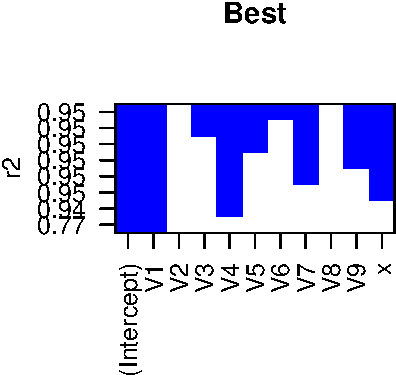
\includegraphics{sol_A3_files/figure-latex/unnamed-chunk-25-1} \end{center}

\begin{Shaded}
\begin{Highlighting}[]
\NormalTok{npred <-}\DecValTok{1}\OperatorTok{:}\DecValTok{8}

\KeywordTok{data.frame}\NormalTok{(}\DataTypeTok{npred =} \DecValTok{1}\OperatorTok{:}\DecValTok{8}\NormalTok{, }
           \DataTypeTok{cp =} \KeywordTok{summary}\NormalTok{(back)}\OperatorTok{$}\NormalTok{cp) }\OperatorTok\StringTok{ }
\StringTok{  }\KeywordTok{ggplot}\NormalTok{(}\KeywordTok{aes}\NormalTok{(npred, cp)) }\OperatorTok{+}
\StringTok{  }\KeywordTok{geom_line}\NormalTok{(}\DataTypeTok{colour =} \StringTok{"blue"}\NormalTok{) }\OperatorTok{+}
\StringTok{  }\KeywordTok{geom_point}\NormalTok{() }\OperatorTok{+}\StringTok{ }
\StringTok{  }\KeywordTok{theme_bw}\NormalTok{()}
\end{Highlighting}
\end{Shaded}

\begin{center}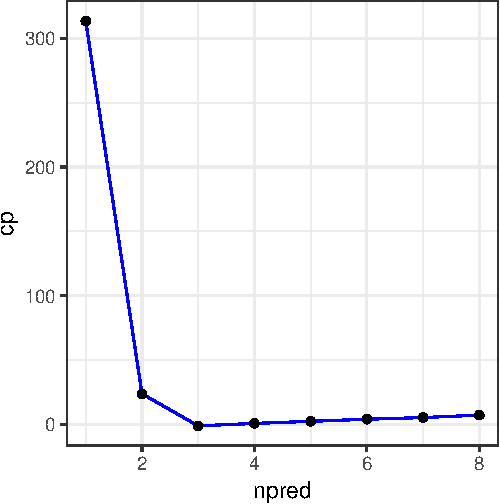
\includegraphics{sol_A3_files/figure-latex/unnamed-chunk-25-2} \end{center}


\end{document}
